\chapter{Digital Logic: Sequential Circuits}

Combinational circuits have no memory: outputs are a function of current
inputs only. To build registers, the PC and memory, we need circuits whose
outputs also depend on their \emph{state}. These are \textbf{sequential
circuits}. The key ingredient is feedback.

\section{Latches}

\subsection{SR latch}

Two cross-coupled NOR gates form an \textbf{SR (set--reset) latch}.

\begin{figure}[H]
\centering
\begin{tikzpicture}[circuit logic US, every circuit symbol/.style={thick}, thick]
  \node[nor gate, inputs=nn] (n1) at (0,1.2) {};
  \node[nor gate, inputs=nn] (n2) at (0,-1.2) {};
  \draw (n1.input 1) -- ++(-1,0) node[left]{$R$};
  \draw (n2.input 2) -- ++(-1,0) node[left]{$S$};
  \draw (n1.output) -- ++(1.2,0) node[right]{$Q$};
  \draw (n2.output) -- ++(1.2,0) node[right]{$\overline{Q}$};
  \draw (n1.output) ++(0.5,0) -- ++(0,-0.8) -- ($(n2.input 1)+(-0.4,0.4)$) -- ++(0,-0.4) -- (n2.input 1);
  \draw (n2.output) ++(0.5,0) -- ++(0,0.8) -- ($(n1.input 2)+(-0.4,-0.4)$) -- ++(0,0.4) -- (n1.input 2);
\end{tikzpicture}
\caption{SR latch from two NOR gates.}
\end{figure}

\begin{center}
\begin{tabular}{cc|cl}
\toprule
$S$ & $R$ & $Q_{next}$ & \\
\midrule
0 & 0 & $Q$ & hold (remember) \\
0 & 1 & 0 & reset \\
1 & 0 & 1 & set \\
1 & 1 & -- & forbidden ($Q = \overline{Q} = 0$, unpredictable after) \\
\bottomrule
\end{tabular}
\end{center}

\subsection{D latch}

To avoid the forbidden state, a \textbf{D latch} derives $S = D\cdot C$ and
$R = \overline{D}\cdot C$ from a data input $D$ and an enable/clock $C$.
When $C = 1$ the latch is \emph{transparent} ($Q$ follows $D$); when $C = 0$
it holds its value.

\section{Clocks and Flip-Flops}

A \textbf{clock} is a periodic signal. Its \emph{period} is the time of one
cycle; the frequency is the reciprocal (a 1\,ns period means 1\,GHz). In
\textbf{edge-triggered} design, state changes only at a clock edge (we use
the rising edge), so all state elements update simultaneously and
combinational logic has a whole cycle to settle in between.

\begin{definition}
A \textbf{D flip-flop} samples $D$ at the rising clock edge and holds that
value in $Q$ until the next rising edge. It can be built from two D latches
in a \emph{master--slave} arrangement: the master is transparent while
$C = 0$, the slave while $C = 1$, so the value passes through only at the
$0 \to 1$ transition.
\end{definition}

\begin{important}[Latch vs flip-flop]
A latch is \emph{level}-sensitive (transparent for the whole time the clock
is high). A flip-flop is \emph{edge}-triggered. Using latches in a loop with
combinational logic can cause a value to race around the loop several times
in one cycle; flip-flops prevent this.
\end{important}

\begin{figure}[H]
\centering
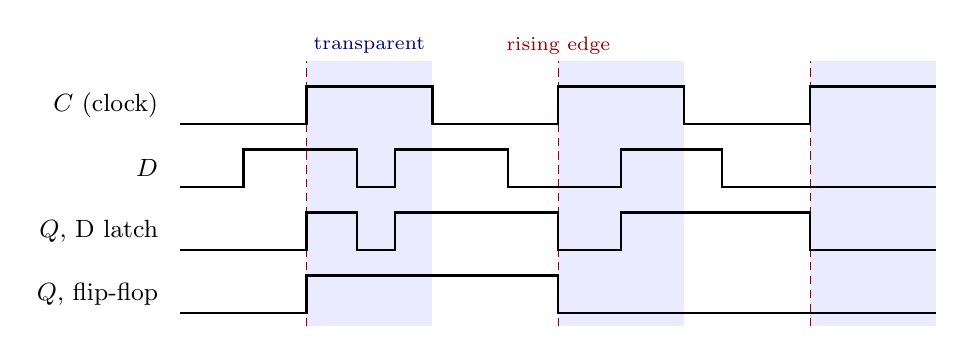
\begin{tikzpicture}[x=1.6cm, y=0.8cm, font=\small]
  \fill[blue!8] (1,-0.2) rectangle (2,4.0);
  \fill[blue!8] (3,-0.2) rectangle (4,4.0);
  \fill[blue!8] (5,-0.2) rectangle (6,4.0);
  \foreach \x in {1,3,5} \draw[red!60!black, densely dashed] (\x,-0.2) -- (\x,4.0);
  \node[anchor=east] at (-0.1,3.3) {$C$ (clock)};
  \node[anchor=east] at (-0.1,2.3) {$D$};
  \node[anchor=east] at (-0.1,1.3) {$Q$, D latch};
  \node[anchor=east] at (-0.1,0.3) {$Q$, flip-flop};
  \draw[thick] (0,3) -- (1,3) -- (1,3.6) -- (2,3.6) -- (2,3) -- (3,3) -- (3,3.6) -- (4,3.6) -- (4,3) -- (5,3) -- (5,3.6) -- (6,3.6);
  \draw[thick] (0,2) -- (0.5,2) -- (0.5,2.6) -- (1.4,2.6) -- (1.4,2) -- (1.7,2) -- (1.7,2.6) -- (2.6,2.6) -- (2.6,2) -- (3.5,2) -- (3.5,2.6) -- (4.3,2.6) -- (4.3,2) -- (6,2);
  \draw[thick] (0,1) -- (1,1) -- (1,1.6) -- (1.4,1.6) -- (1.4,1) -- (1.7,1) -- (1.7,1.6) -- (3,1.6) -- (3,1) -- (3.5,1) -- (3.5,1.6) -- (5,1.6) -- (5,1) -- (6,1);
  \draw[thick] (0,0) -- (1,0) -- (1,0.6) -- (3,0.6) -- (3,0) -- (6,0);
  \node[font=\scriptsize, blue!50!black] at (1.5,4.25) {transparent};
  \node[font=\scriptsize, red!60!black] at (3,4.25) {rising edge};
\end{tikzpicture}
\caption{A D latch (level-sensitive) passes every change of $D$ while the
clock is high (shaded); a D flip-flop only samples $D$ at the rising edges
(dashed), so it ignores the short pulse in $D$ during the first high phase.}
\end{figure}

\paragraph{Timing constraints.} The input must be stable for a
\emph{setup time} before the edge and a \emph{hold time} after it; the output
changes a \emph{clock-to-Q} delay after the edge. Therefore
\[
T_{clock} \ge t_{clk\to Q} + t_{\text{critical path}} + t_{setup}.
\]

\begin{figure}[H]
\centering
\begin{tikzpicture}[x=1cm, y=0.8cm, font=\small, >=Stealth]
  % clock
  \draw[thick] (0,2) -- (1,2) -- (1,2.6) -- (5,2.6) -- (5,2) -- (9,2) -- (9,2.6) -- (10.5,2.6);
  \node[anchor=east] at (-0.1,2.3) {clock};
  % register output Q and combinational logic output
  \draw[thick] (0,1) -- (1.6,1) (0,1.6) -- (1.6,1.6);
  \draw[thick] (1.6,1) -- (1.8,1.6) (1.6,1.6) -- (1.8,1) ;
  \draw[thick] (1.8,1) -- (10.5,1) (1.8,1.6) -- (10.5,1.6);
  \node[anchor=east] at (-0.1,1.3) {$Q$};
  \draw[thick] (0,0) -- (6.4,0) (0,0.6) -- (6.4,0.6);
  \fill[gray!25] (1.8,0) -- (6.4,0) -- (6.6,0.3) -- (6.4,0.6) -- (1.8,0.6) -- cycle;
  \draw[thick] (6.4,0) -- (6.6,0.3) -- (6.4,0.6) (6.6,0.3) -- (6.8,0) -- (10.5,0) (6.6,0.3) -- (6.8,0.6) -- (10.5,0.6);
  \node[font=\scriptsize] at (4.1,0.3) {logic settling};
  \node[anchor=east] at (-0.1,0.3) {next $D$};
  % edges and annotations
  \draw[densely dashed] (1,-0.3) -- (1,3) (9,-0.3) -- (9,3);
  \draw[<->] (1,-0.6) -- node[below, font=\scriptsize]{$t_{clk\to Q}$} (1.8,-0.6);
  \draw[<->] (1.8,-0.6) -- node[below, font=\scriptsize]{$t_{\text{critical path}}$} (6.8,-0.6);
  \draw[<->] (6.8,-0.6) -- node[below, font=\scriptsize]{slack} (8.2,-0.6);
  \fill[red!20] (8.2,-0.1) rectangle (9,0.7);
  \fill[orange!25] (9,-0.1) rectangle (9.5,0.7);
  \draw[thick] (6.8,0) -- (10.5,0) (6.8,0.6) -- (10.5,0.6);
  \draw[<->] (8.2,-0.6) -- node[below, font=\scriptsize]{$t_{setup}$} (9,-0.6);
  \draw[<->] (9,-0.6) -- node[below right=-1pt, font=\scriptsize]{$t_{hold}$} (9.5,-0.6);
  \draw[<->] (1,3.2) -- node[above, font=\scriptsize]{$T_{clock}$} (9,3.2);
\end{tikzpicture}
\caption{One clock cycle: the register output changes $t_{clk\to Q}$ after
the edge, the logic settles along its critical path, and the new $D$ must be
stable from $t_{setup}$ before the next edge until $t_{hold}$ after it.}
\end{figure}

\subsection{Other flip-flops}
\begin{itemize}
  \item \textbf{JK}: like SR, but $J = K = 1$ toggles.
  \item \textbf{T}: toggles when $T = 1$, holds when $T = 0$. Useful for
    counters.
\end{itemize}

\section{Registers and Register Files}

An $n$-bit \textbf{register} is $n$ D flip-flops sharing a clock. Adding a
\textbf{write enable}: a mux in front of each flip-flop feeds back $Q$ when
the enable is 0, so the register keeps its value.

\begin{definition}
The MIPS \textbf{register file} holds 32 registers of 32 bits. It has
\begin{itemize}
  \item two read ports: 5-bit read register numbers select outputs via two
    32-to-1 muxes (of 32-bit buses);
  \item one write port: a 5-bit write register number goes through a
    5-to-32 decoder, ANDed with \code{RegWrite}, to enable exactly one
    register; the write data is presented to all registers.
\end{itemize}
Reads are combinational; the write happens at the clock edge.
\end{definition}

\begin{figure}[H]
\centering
\begin{tikzpicture}[>=Stealth, thick, font=\small]
  \node[draw, minimum width=3.2cm, minimum height=3.6cm, align=center] (rf) at (0,0) {Register file\\[2pt]{\scriptsize 32 $\times$ 32 bits}};
  \foreach \y/\lab/\w in {1.3/Read reg 1/5, 0.6/Read reg 2/5, -0.1/Write reg/5, -1.0/Write data/32} {
    \draw[->] (-3.4,\y) -- node[above, font=\scriptsize, pos=0.4]{\lab} (-1.6,\y);
    \draw (-2.9,\y-0.1) -- (-2.8,\y+0.1);
    \node[font=\tiny, below] at (-2.85,\y-0.05) {\w};
  }
  \foreach \y/\lab in {0.9/Read data 1, -0.6/Read data 2} {
    \draw[->] (1.6,\y) -- node[above, font=\scriptsize, pos=0.6]{\lab} (3.6,\y);
    \draw (2.2,\y-0.1) -- (2.3,\y+0.1);
    \node[font=\tiny, below] at (2.25,\y-0.05) {32};
  }
  \draw[<-] (0,1.8) -- (0,2.4) node[above, font=\scriptsize]{RegWrite};
  \draw (-0.25,-1.8) -- (0,-1.55) -- (0.25,-1.8);
  \draw[<-] (0,-1.8) -- (0,-2.3) node[below, font=\scriptsize]{clock};
\end{tikzpicture}
\caption{Interface of the MIPS register file: two 5-bit read register
numbers select two 32-bit outputs; the write port writes \emph{Write data}
into \emph{Write reg} at the clock edge when \code{RegWrite} = 1.}
\end{figure}

Other register types: \textbf{shift registers} (each flip-flop's input is
its neighbour's output) and \textbf{counters} (register + incrementer).

\section{Finite State Machines}

\begin{definition}
A \textbf{finite state machine (FSM)} consists of a state register, next-state
logic (combinational; inputs: current state and inputs) and output logic.
\begin{itemize}
  \item \textbf{Moore} machine: outputs depend only on the current state.
  \item \textbf{Mealy} machine: outputs depend on state and inputs.
\end{itemize}
\end{definition}

\begin{figure}[H]
\centering
\begin{tikzpicture}[>=Stealth, thick, font=\small,
  blk/.style={draw, rounded corners, align=center, minimum height=1.3cm, text width=1.8cm}]
  \node[blk] (ns) at (0,0) {Next-state\\logic};
  \node[draw, fill=gray!20, minimum height=1.3cm, minimum width=1.2cm, align=center] (sr) at (3.4,0) {State\\reg};
  \node[blk] (out) at (7.0,0) {Output\\logic};
  \draw[->] (-2.4,0.3) node[left]{inputs} -- ($(ns.west)+(0,0.3)$);
  \draw[->] (ns) -- node[above, font=\scriptsize]{next state} (sr);
  \draw[->] (sr) -- node[above, font=\scriptsize, pos=0.6]{current state} (out);
  \draw[->] (out) -- (8.8,0) node[right]{outputs};
  \draw[->] ($(sr.east)+(0.2,0)$) -- ++(0,-1.3) -| ($(ns.west)+(-0.4,-0.3)$) -- ($(ns.west)+(0,-0.3)$);
  \fill ($(sr.east)+(0.2,0)$) circle (1.5pt);
  \draw[->, densely dashed] (-1.8,0.3) -- (-1.8,1.3) -| node[pos=0.25, above, font=\scriptsize]{Mealy only} (out.north);
  \fill (-1.8,0.3) circle (1.5pt);
  \draw (3.1,-0.65) -- (3.4,-0.4) -- (3.7,-0.65);
\end{tikzpicture}
\caption{Structure of a synchronous FSM. In a Moore machine the outputs
depend only on the state; a Mealy machine also feeds the inputs to the
output logic (dashed).}
\end{figure}

Design procedure:
\begin{enumerate}
  \item Draw the state diagram.
  \item Choose a state encoding (binary, or one-hot with one flip-flop per state).
  \item Write the state transition table and the output table.
  \item Derive next-state and output equations (K-maps).
  \item Build with flip-flops and gates.
\end{enumerate}

\begin{example}[Sequence detector]
Output 1 when the last two input bits were both 1 (Moore machine).
States: $S_0$ (last bit 0 / start), $S_1$ (seen one 1), $S_2$ (seen
$\ge$ two 1s, output 1).

\begin{figure}[H]
\centering
\begin{tikzpicture}[->, >=Stealth, node distance=2.8cm, auto, thick,
  every state/.style={minimum size=1.1cm}]
  \node[state, initial] (s0) {$S_0/0$};
  \node[state, right of=s0] (s1) {$S_1/0$};
  \node[state, right of=s1] (s2) {$S_2/1$};
  \path (s0) edge[loop above] node{0} (s0)
             edge node{1} (s1)
        (s1) edge node{1} (s2)
             edge[bend left] node{0} (s0)
        (s2) edge[loop above] node{1} (s2)
             edge[bend left=45] node{0} (s0);
\end{tikzpicture}
\end{figure}

With encoding $S_0 = 00$, $S_1 = 01$, $S_2 = 10$ (state bits $Q_1Q_0$,
input $x$):
\begin{center}
\begin{tabular}{cc|c|cc|c}
\toprule
$Q_1$ & $Q_0$ & $x$ & $D_1$ & $D_0$ & $z$ \\
\midrule
0&0&0&0&0&0\\
0&0&1&0&1&0\\
0&1&0&0&0&0\\
0&1&1&1&0&0\\
1&0&0&0&0&1\\
1&0&1&1&0&1\\
\bottomrule
\end{tabular}
\end{center}
State 11 is unused (don't care). Using don't cares:
$D_1 = x(Q_1 + Q_0)$, $D_0 = x\overline{Q_1}\,\overline{Q_0}$, $z = Q_1$.
\end{example}

FSMs reappear as the control unit of the multi-cycle processor.

\section{Memory}

\begin{itemize}
  \item \textbf{SRAM}: each bit is a latch-like cell (6 transistors). Fast,
    no refresh, expensive: used for caches and register files.
  \item \textbf{DRAM}: each bit is a capacitor + 1 transistor. Dense and
    cheap but slower, and must be periodically refreshed because charge
    leaks: used for main memory.
\end{itemize}
A memory with $2^k$ words is addressed through a decoder (row select) and
muxes (column select).

\section*{Summary}
\begin{itemize}
  \item Feedback gives memory: SR latch $\to$ D latch (level-sensitive)
    $\to$ D flip-flop (edge-triggered, master--slave).
  \item Clock period $\ge$ clk-to-Q + critical path + setup.
  \item Register = flip-flops + write enable; register file = 32 registers,
    2 read ports (muxes), 1 write port (decoder).
  \item FSM = state register + next-state logic + output logic; Moore vs
    Mealy; design via state table and K-maps.
  \item SRAM fast/expensive (caches), DRAM dense/slow (main memory).
\end{itemize}
